%\vspace{10pt}
\section{Non-linearity}\label{sec:scale}
%\section{Non-linearity and Write Current Scaling}\label{sec:scale}
\vspace{6pt} \emph{Non-linearity of the ReRAM Cell.} \vspace{6pt}

\begin{figure}[!b]
\centering
  % Requires \usepackage{graphicx}
  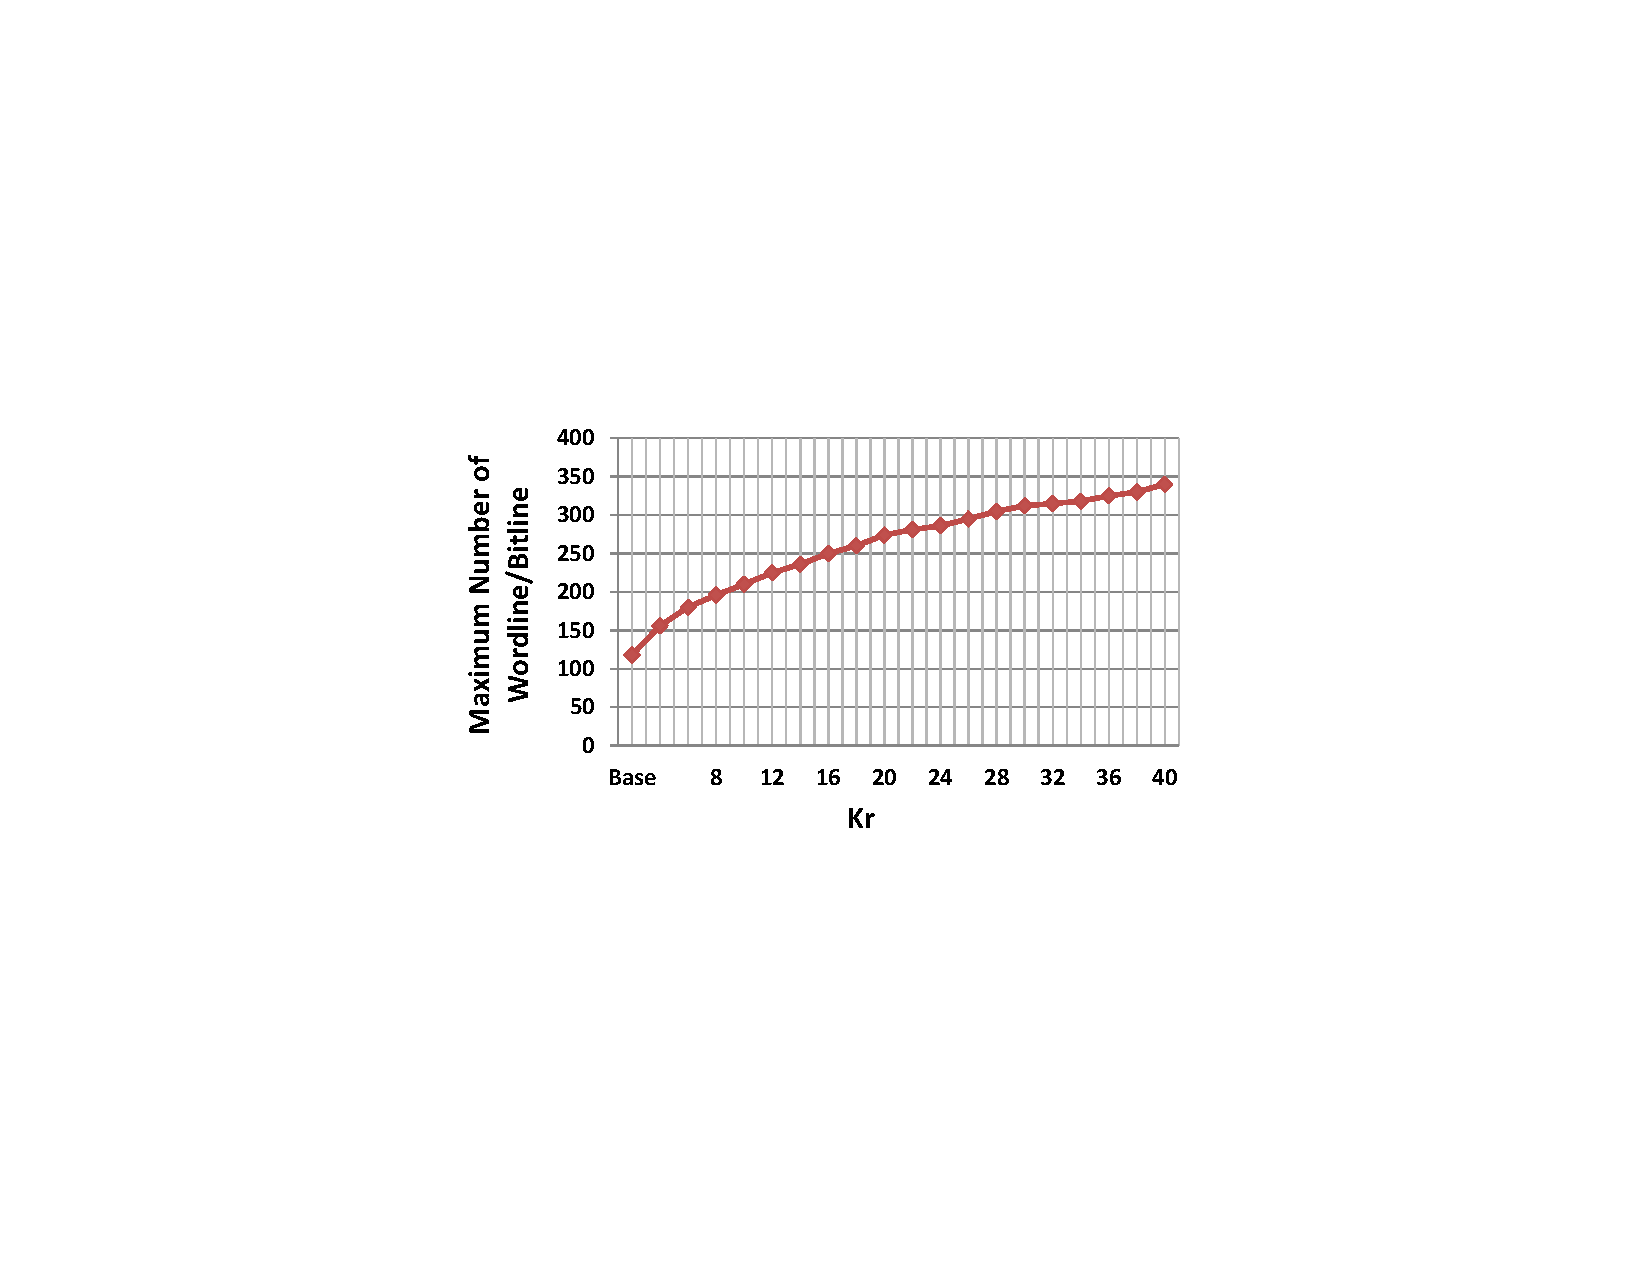
\includegraphics[width=0.4\textwidth]{./figures/non_linear_f}\\
  \caption{The maximum array size with different non-linearity coefficient.}\label{fig:non_linear}
\end{figure}
One of the most distinct features of ReRAM is its non-linearity. For
example, the non-linearity of memristor-based ReRAM is observed at LRS
when the resistance of the memristor cell is not constant but varies with
the applied voltage. The non-linearity coefficient is defined as:
$K_r(p,V) = p \times R(V/p)/R(V)$, where $R(V/p)$ and $R(V)$ are the
equivalent resistance of the memristor biased at $V/p$ and
$V$~\cite{memristor:Cong}. Normally, the $K_r(p,V)$ value for
memristor-based ReRAM is larger than 20, meaning that the resistance of a
half-biased  cell is at least 10 times larger than a full-biased cell.
Clearly, the ReRAM cell with a larger non-linearity coefficient results in
a better memory cell since the current in the sneak path will be
significantly reduced. In addition, the increased resistance at
half-selected and unselected cells can also mitigate the voltage drop
along the activated wordline and bitline. Figure~\ref{fig:non_linear}
shows the influence of different non-linearity coefficients on the array
size requirements for one bit HWHB writing scheme. In this figure, the
maximum array size increases from $112 \times 112$ to $340 \times 340$
when the non-linearity coefficient $K_r$ increases from 1 to 10.
Similarly, the non-linearity can also increase the maximum array size for
other write schemes.


Moreover, the non-linearity can also reduce the energy consumption and
area overheads of the cross-point array. For example, consider a $128
\times 128$ array. As shown in Figure~\ref{fig:non_linear_energy}, the
energy consumption for the write operation decreases dramatically with the
increase of non-linearity coefficient $K_r$. As $K_r$ increases from 1 to
40, the write energy is reduced by 98.3\%. The driven current requirement
is shown in Figure~\ref{fig:area_all}(a), and the corresponding area
overheads of the voltage drivers are compared to the array size at
Figure~\ref{fig:area_all}(b). The baseline design is unacceptable because
the area of voltage drivers is about 11.6 times larger than the area of
the cross-point array. In this case, the area efficiency of ReRAM's $4F^2$
cell size will be offset by the extremely huge area overhead of the
voltage drivers. However, with the increase of non-linearity, the area of
voltage drivers becomes comparable to the array area. Therefore, we can
conclude that, the ReRAM cells with a small non-linearity coefficient are
not suitable for the cross-point structure based memory array. Next, we
study the area overhead of multi-bit write. Figure~\ref{fig:Area_kr20}
shows the normalized areas of the voltage drivers for one bit and
multi-bit write operations. As mentioned, multi-bit write operations
require larger driven current. Therefore, the area of voltage drivers for
multi-bit write operations are much larger than that for one bit write
operations. Finally, normalized areas of the one bit and multi-bit write
operations have opposite trends as the array size increases. Normalized
area for one bit write operation increases with the array size. On the
contrary, normalized area for multi-bit write decreases as the array size
increase.

\begin{figure}%[!t]
\centering
  % Requires \usepackage{graphicx}
  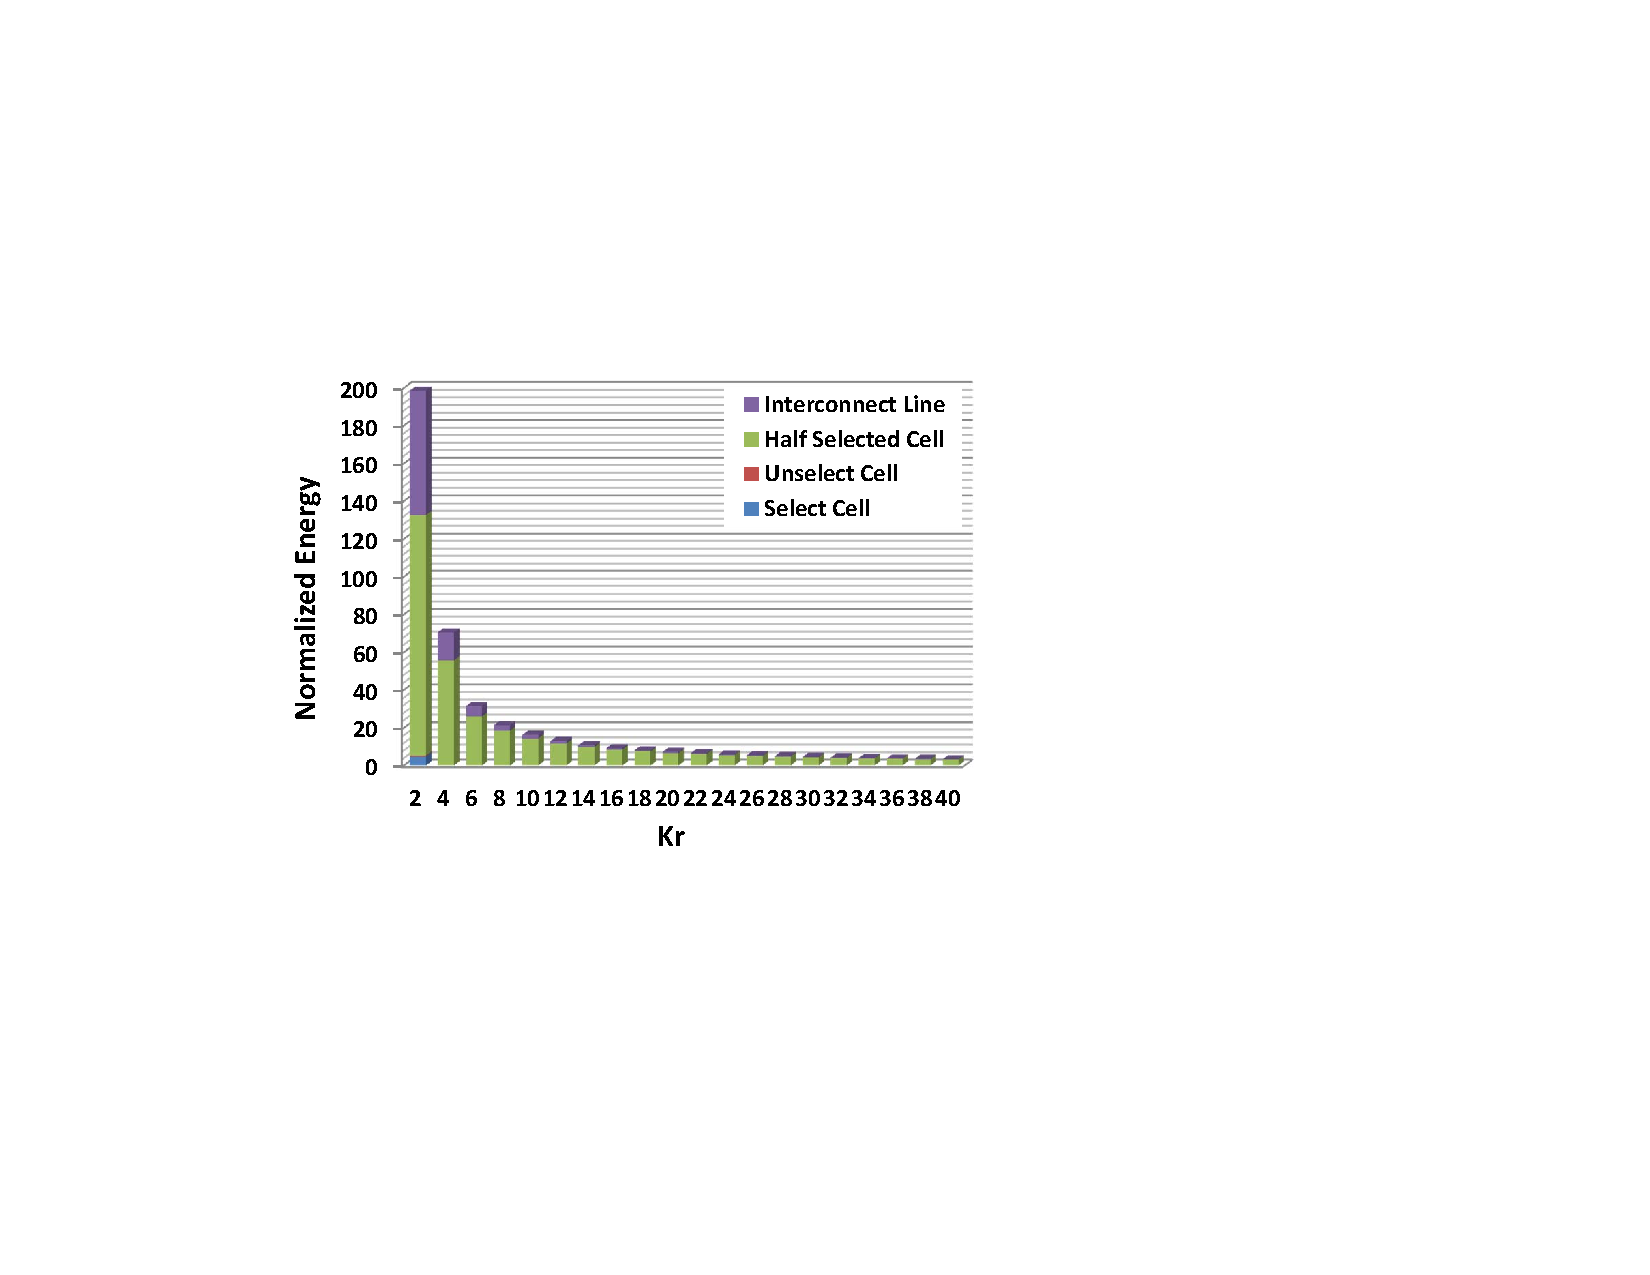
\includegraphics[width=0.38\textwidth]{./figures/non_linear_energy.pdf}\\
  \caption{The normalized energy consumption with non-linear ReRAM cells.}\label{fig:non_linear_energy}
\end{figure}

%\begin{figure}%[!t]
%\centering
%  % Requires \usepackage{graphicx}
%  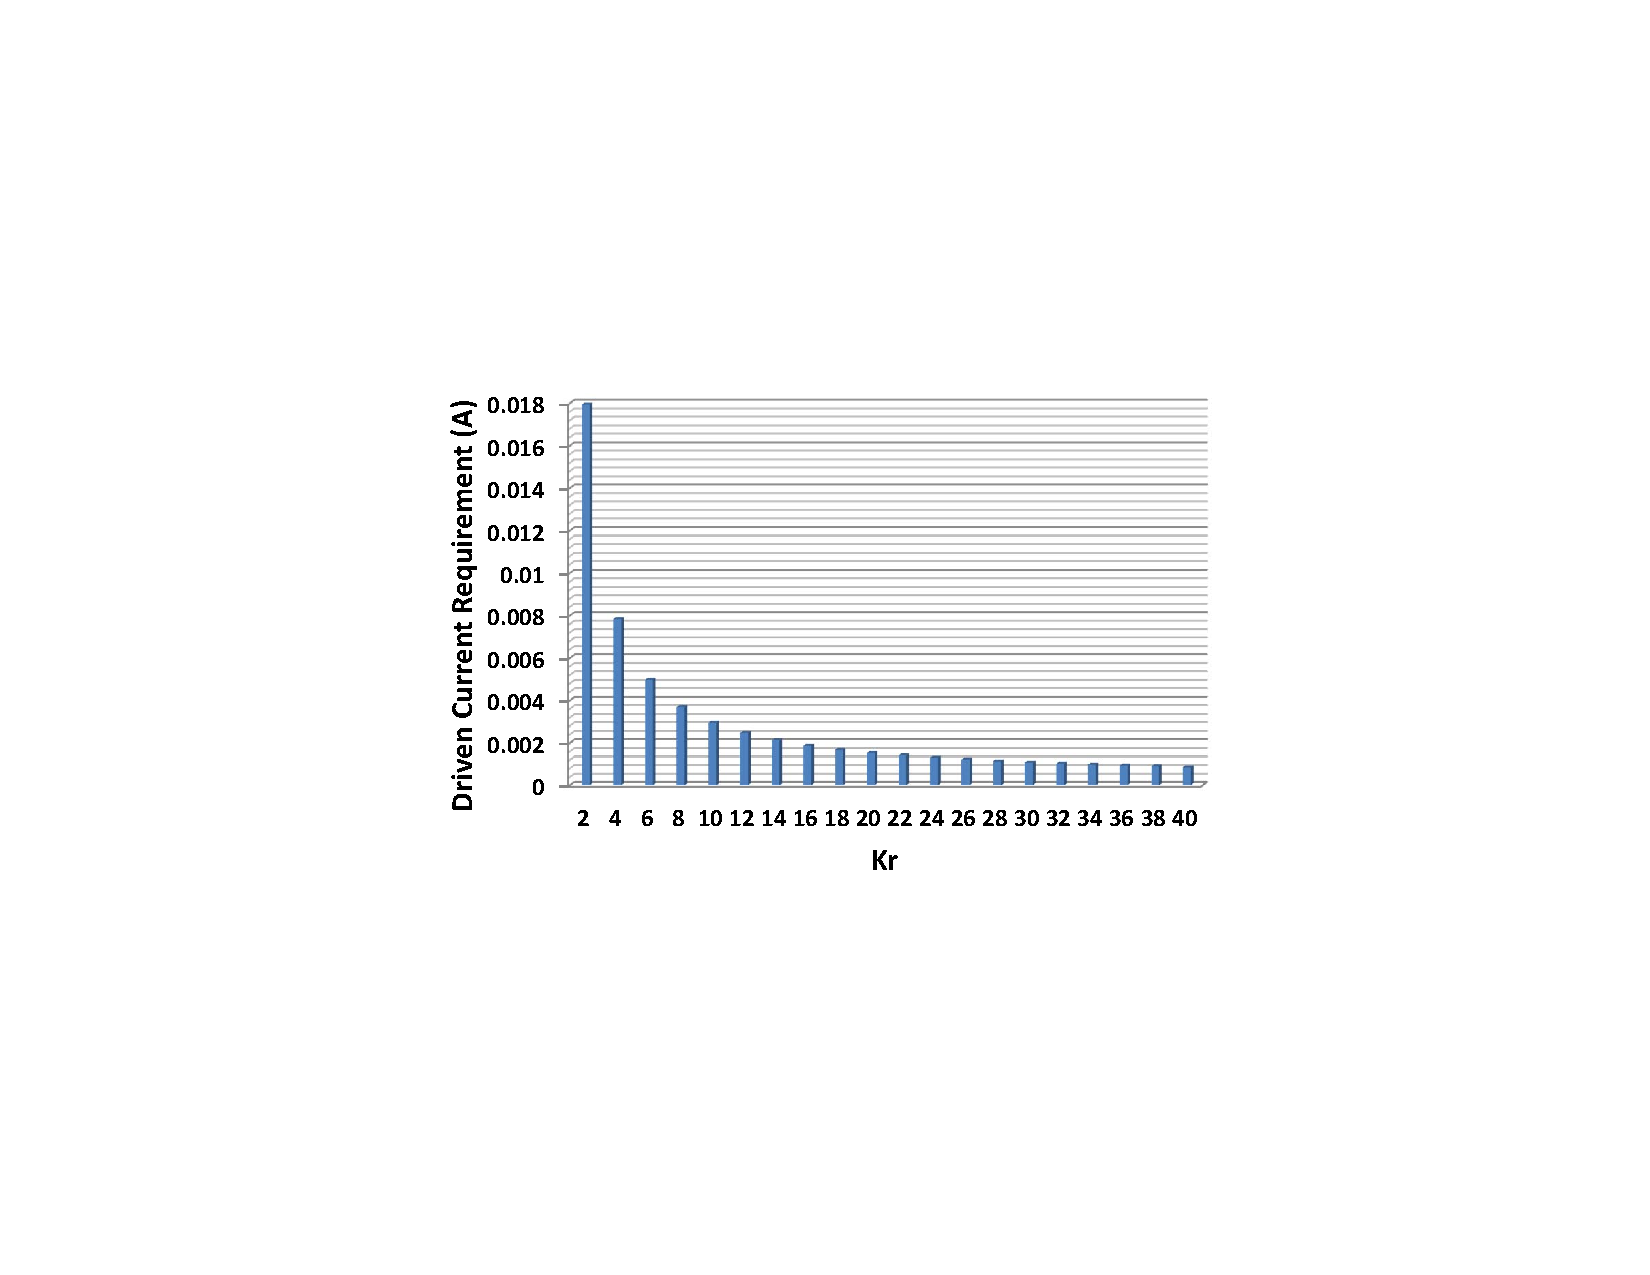
\includegraphics[width=0.4\textwidth]{./figures/non_linear_I.pdf}\\
%  \caption{The}\label{fig:non_linear_I}
%\end{figure}
%
%\begin{figure}%[!t]
%\centering
%  % Requires \usepackage{graphicx}
%  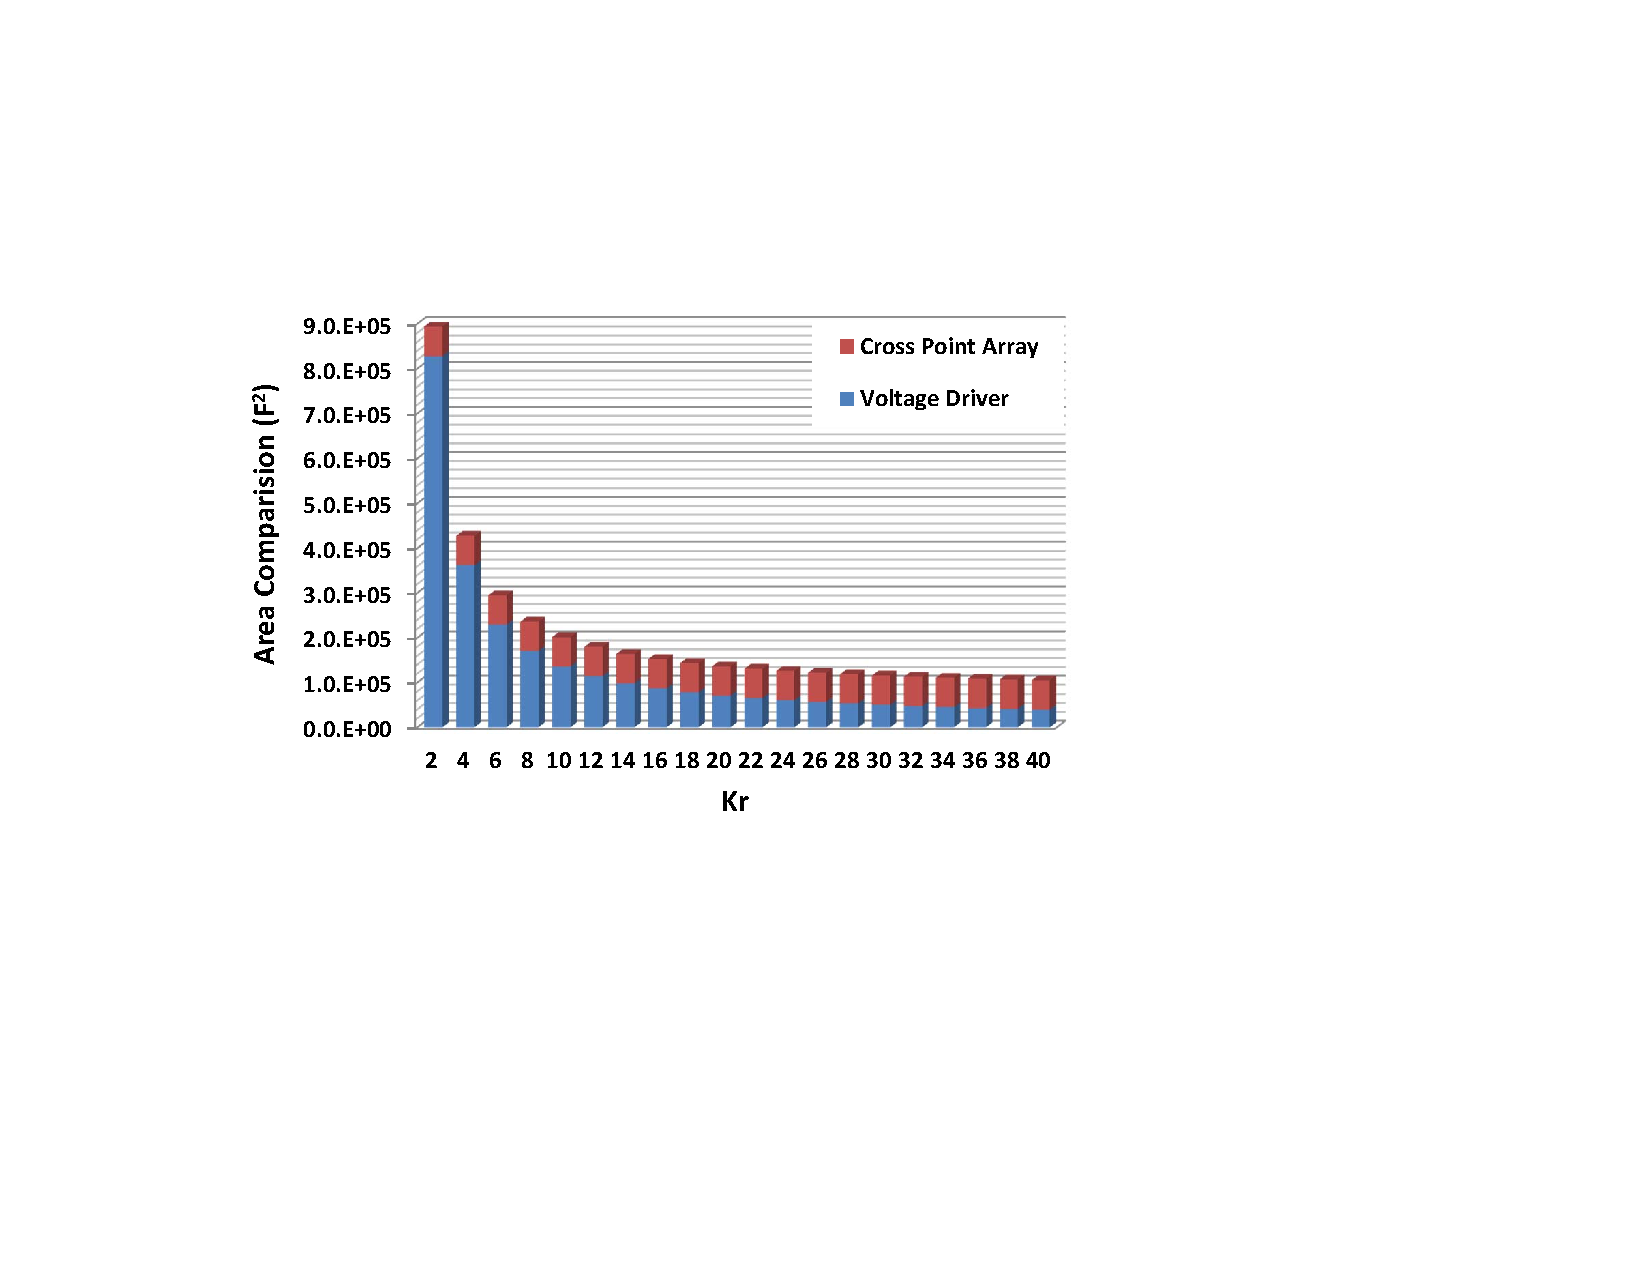
\includegraphics[width=0.4\textwidth]{./figures/non_linear_ara.pdf}\\
%  \caption{The}\label{fig:non_linear_ara}
%\end{figure}
\begin{figure}%[!t]
\centering
  % Requires \usepackage{graphicx}
  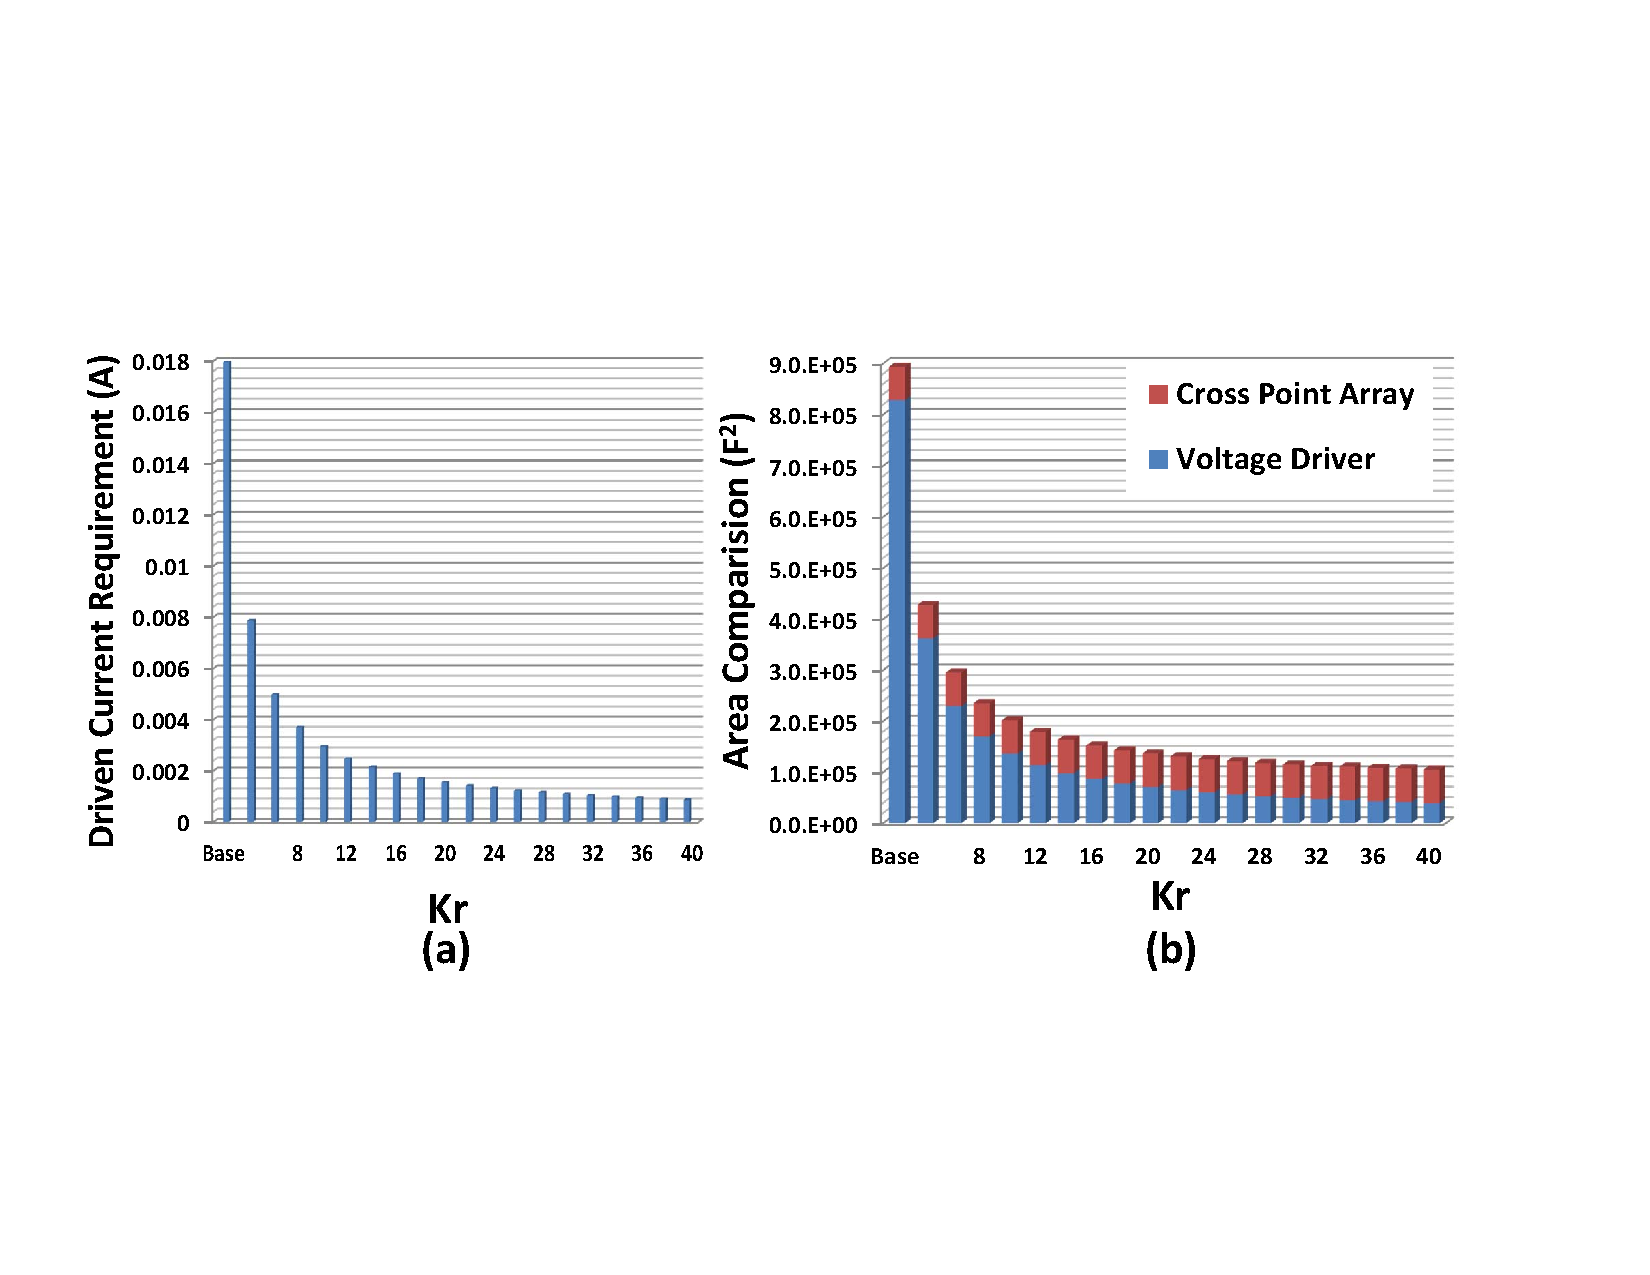
\includegraphics[width=0.5\textwidth]{./figures/area_all.pdf}\\
  \vspace{-5pt}
  \caption{The driven current requirements and area overheads with different non-linearity coefficients}\label{fig:area_all}
 \vspace{-15pt}
\end{figure}


\begin{figure}%[!t]
\centering
  % Requires \usepackage{graphicx}
  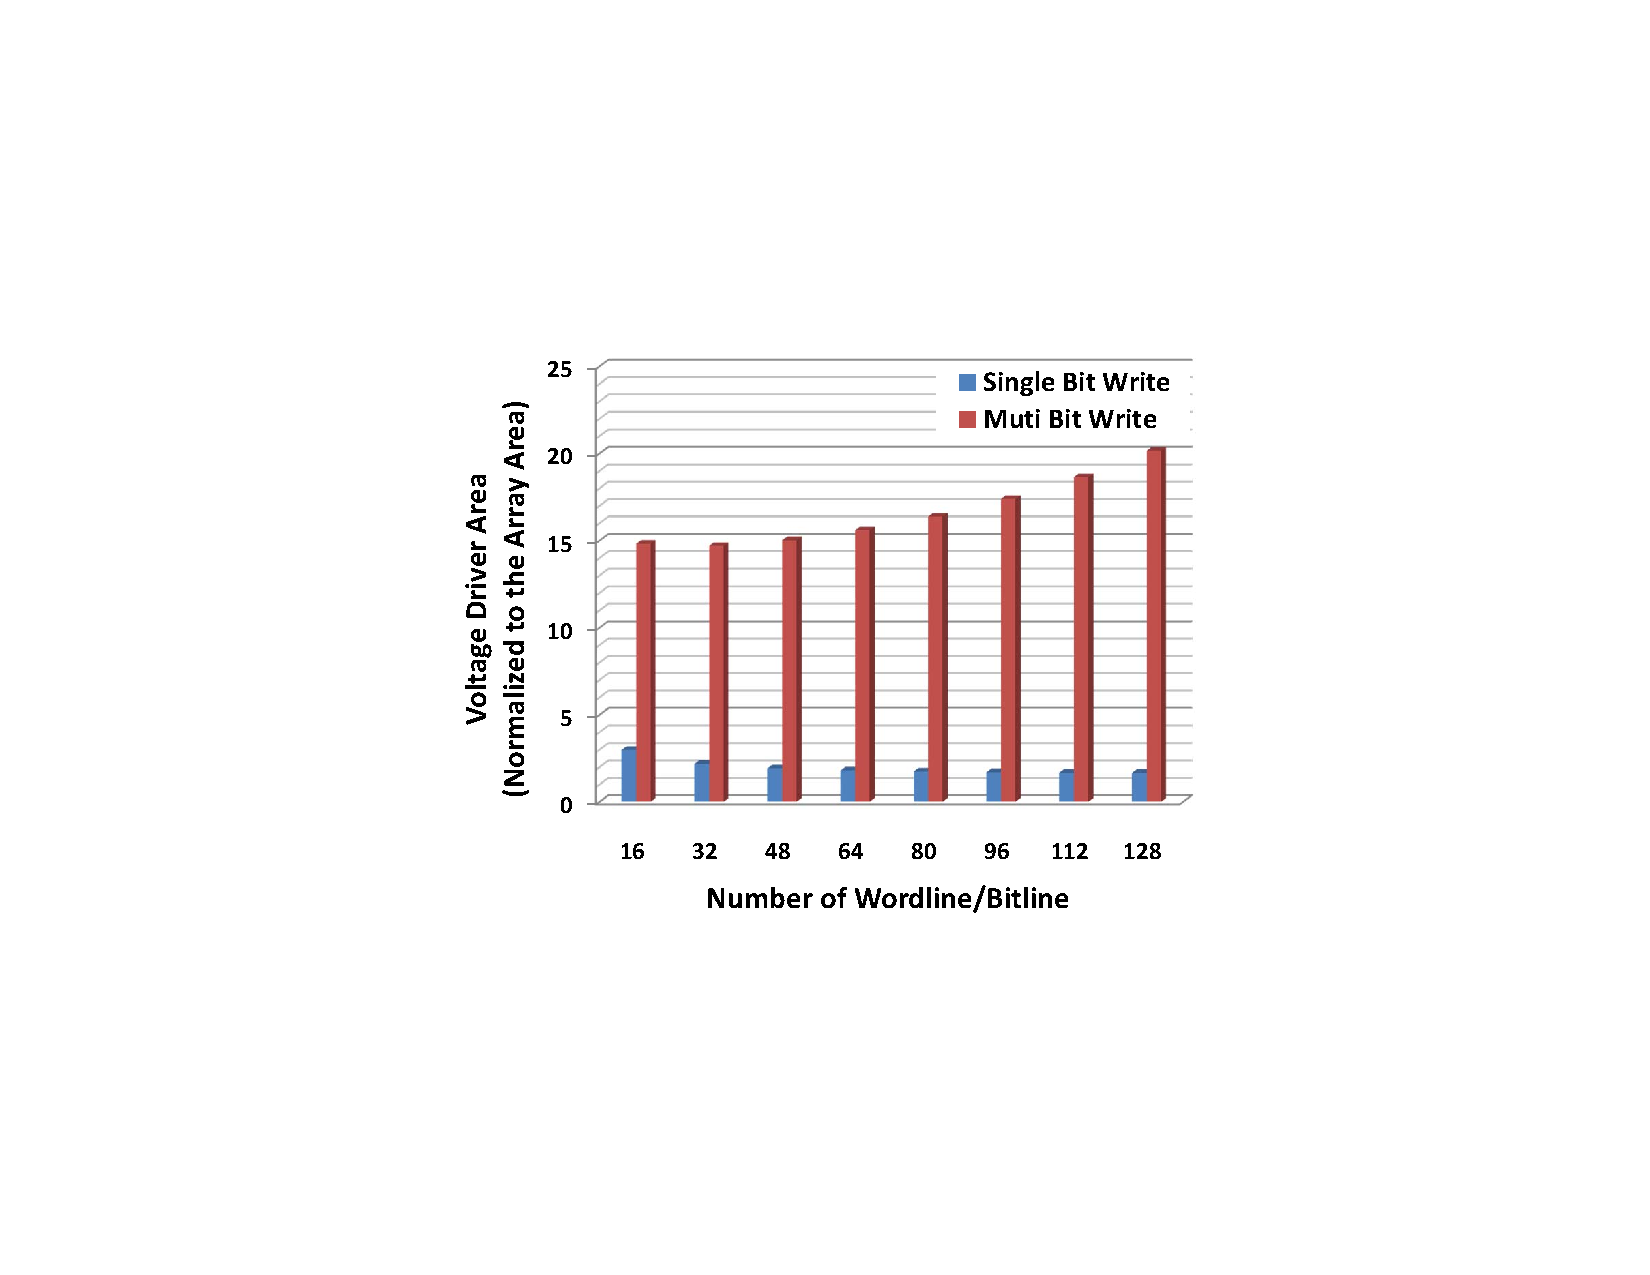
\includegraphics[width=0.35\textwidth]{./figures/Area_kr20_f.pdf}\\
  \caption{The normalized area overhead of voltage drivers ($K_r=20$, the areas are normalized to the area of cross-point array). }\label{fig:Area_kr20}
\end{figure}

\subsection{Read Operation}
In this section we applied the similar sensing scheme as
\cite{crossbar_TED_2010} and \cite{crossbar_NANO08_Flocke}. In order to
read cell $R_{i,j}$, the $i^{th}$ wordline is biased at $V_{READ}$ and all
of the other wordlines and bitlines are grounded. Then the state of the
selected cell is read out by measuring the voltage across $R_s$. The
energy consumption for read operation can be analyzed by the same way as
that of the write operation. Since the read voltage is much smaller than
write voltage, the read energy is expected at least one order smaller than
write operation. Additionally, since the read voltage/current is much
lower than the write, we believe that the voltage drivers can always
provide enough current for the read operation if they meet the current
requirement for write operation. Therefore, we can conclude that the area
overhead of voltage drivers is determined by the write current. However,
the reliability of read operation is different from the write operation.
The read reliability is determined by the voltage swing for reading HRS
and LRS cells. Figure~\ref{fig:sense_margin} (a) shows the voltage swing
with different array sizes and $K_r$ values. Large array sizes and large
non-linearity are harmful to the voltage swing: on the one hand, a larger
array has more sneak paths, making the output voltage very sensitive to
the data pattern of unselected cells; on the other hand, the non-linearity
increases the resistance of LRS and therefore the resistance difference
between HRS and LRS cells is reduced. In order to improve the reliability
of the read operation, a two-step sensing scheme can be applied, which
senses the current of an unselected cell first, then the overall current
is sensed, and after that the current difference is converted to the
output voltage. The voltage swing of this two-step sensing scheme is shown
in Figure~\ref{fig:sense_margin} (b). By using this two-step sensing
schemes, the voltage swing for a given array size and non-linearity
coefficient is doubled.

%\begin{figure}%[!t]
%\centering
%  % Requires \usepackage{graphicx}
%  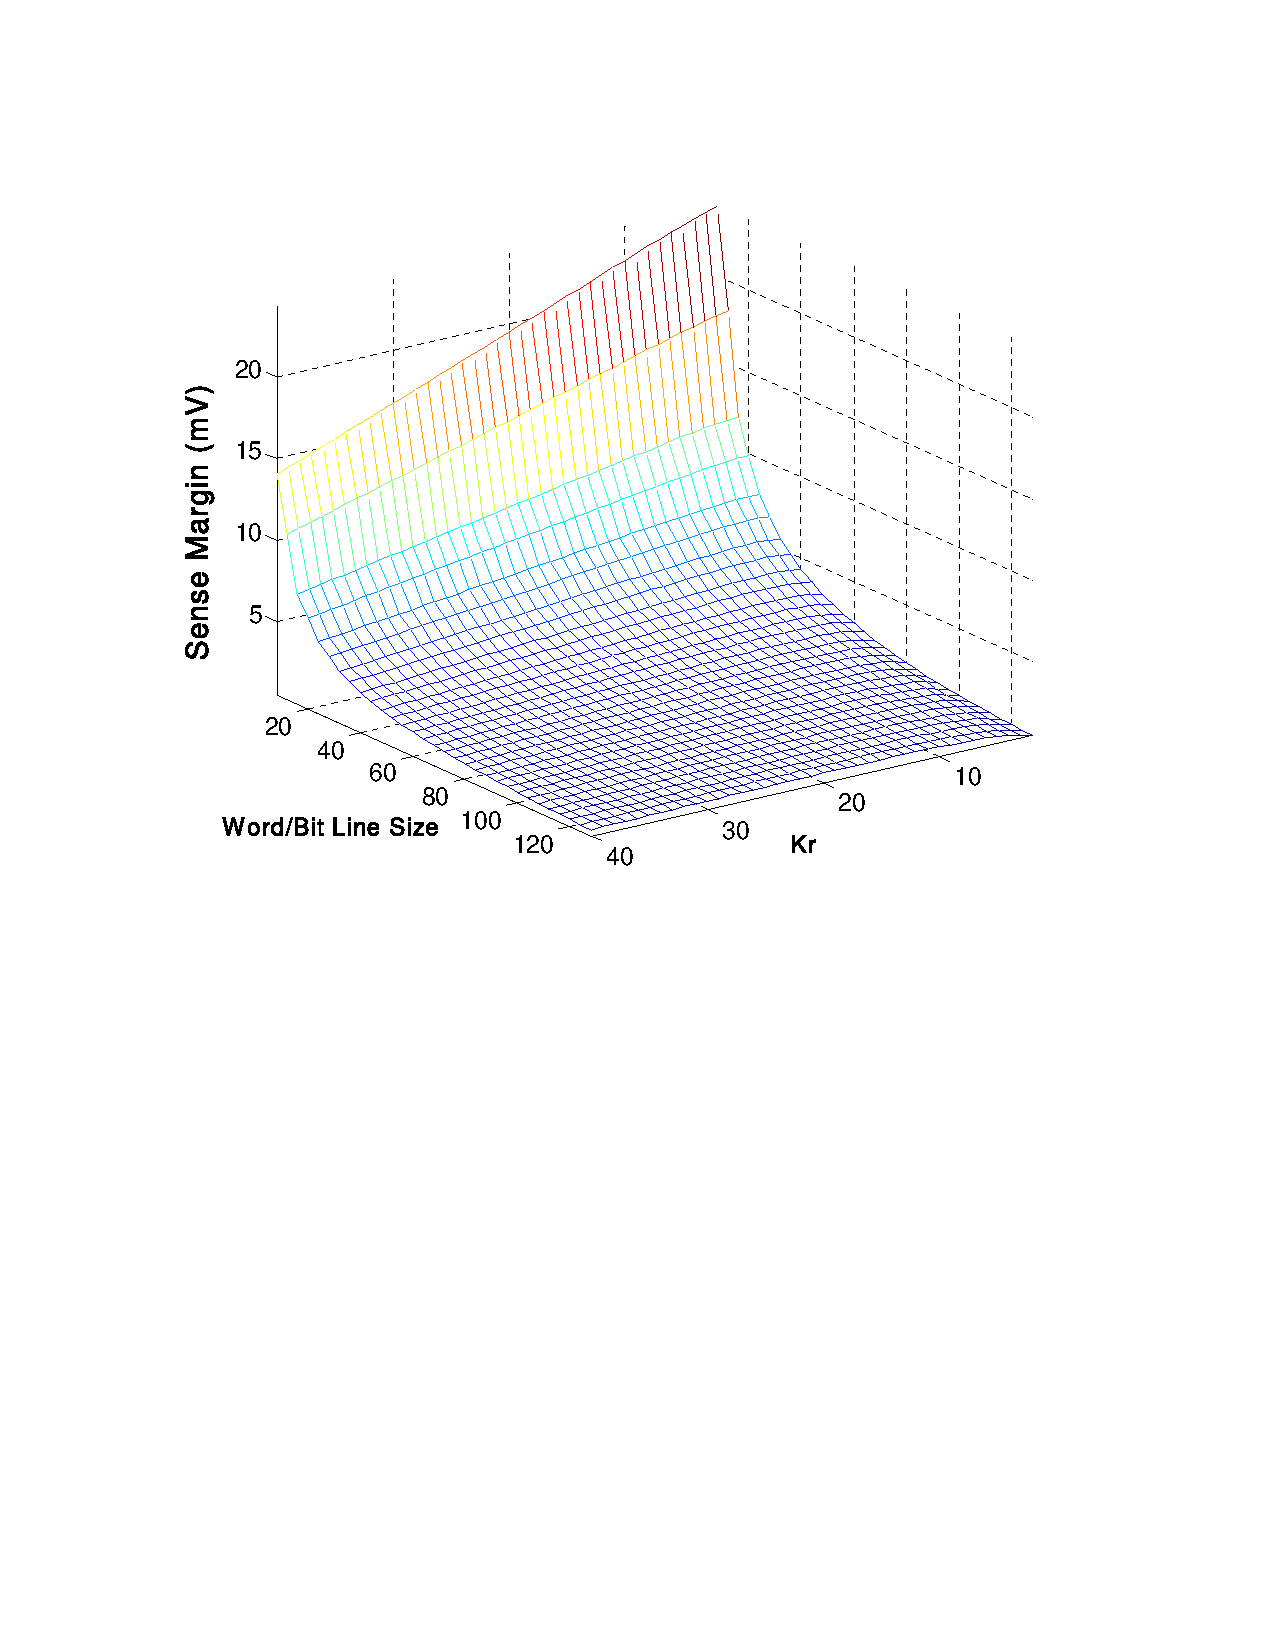
\includegraphics[width=0.45\textwidth]{./figures/margin.pdf}
%  \caption{The}\label{fig:margin}
%\end{figure}
%
%\begin{figure}%[!t]
%\centering
%  % Requires \usepackage{graphicx}
%  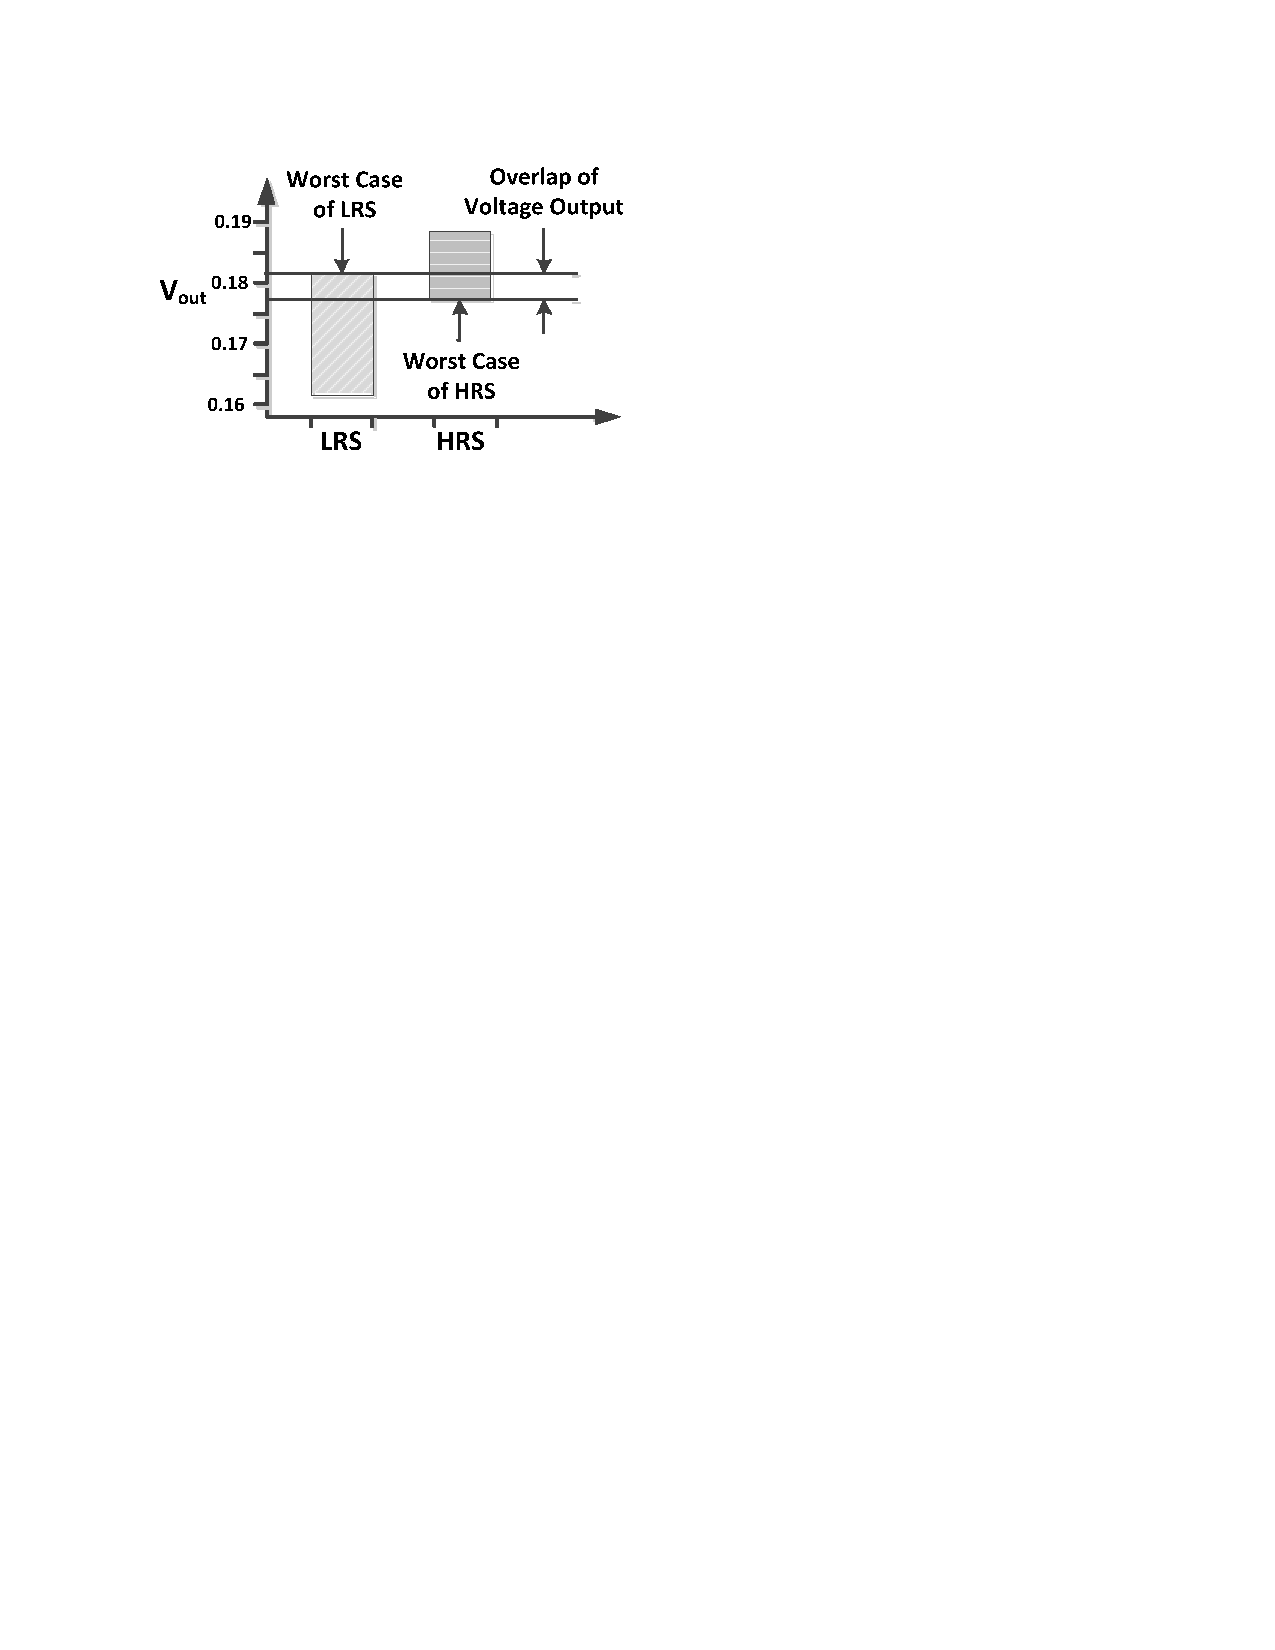
\includegraphics[width=0.4\textwidth]{./figures/overlap.pdf}\\
%  \caption{The}\label{fig:overlap}
%\end{figure}

%
%\begin{figure}%[!t]
%\centering
%  % Requires \usepackage{graphicx}
%  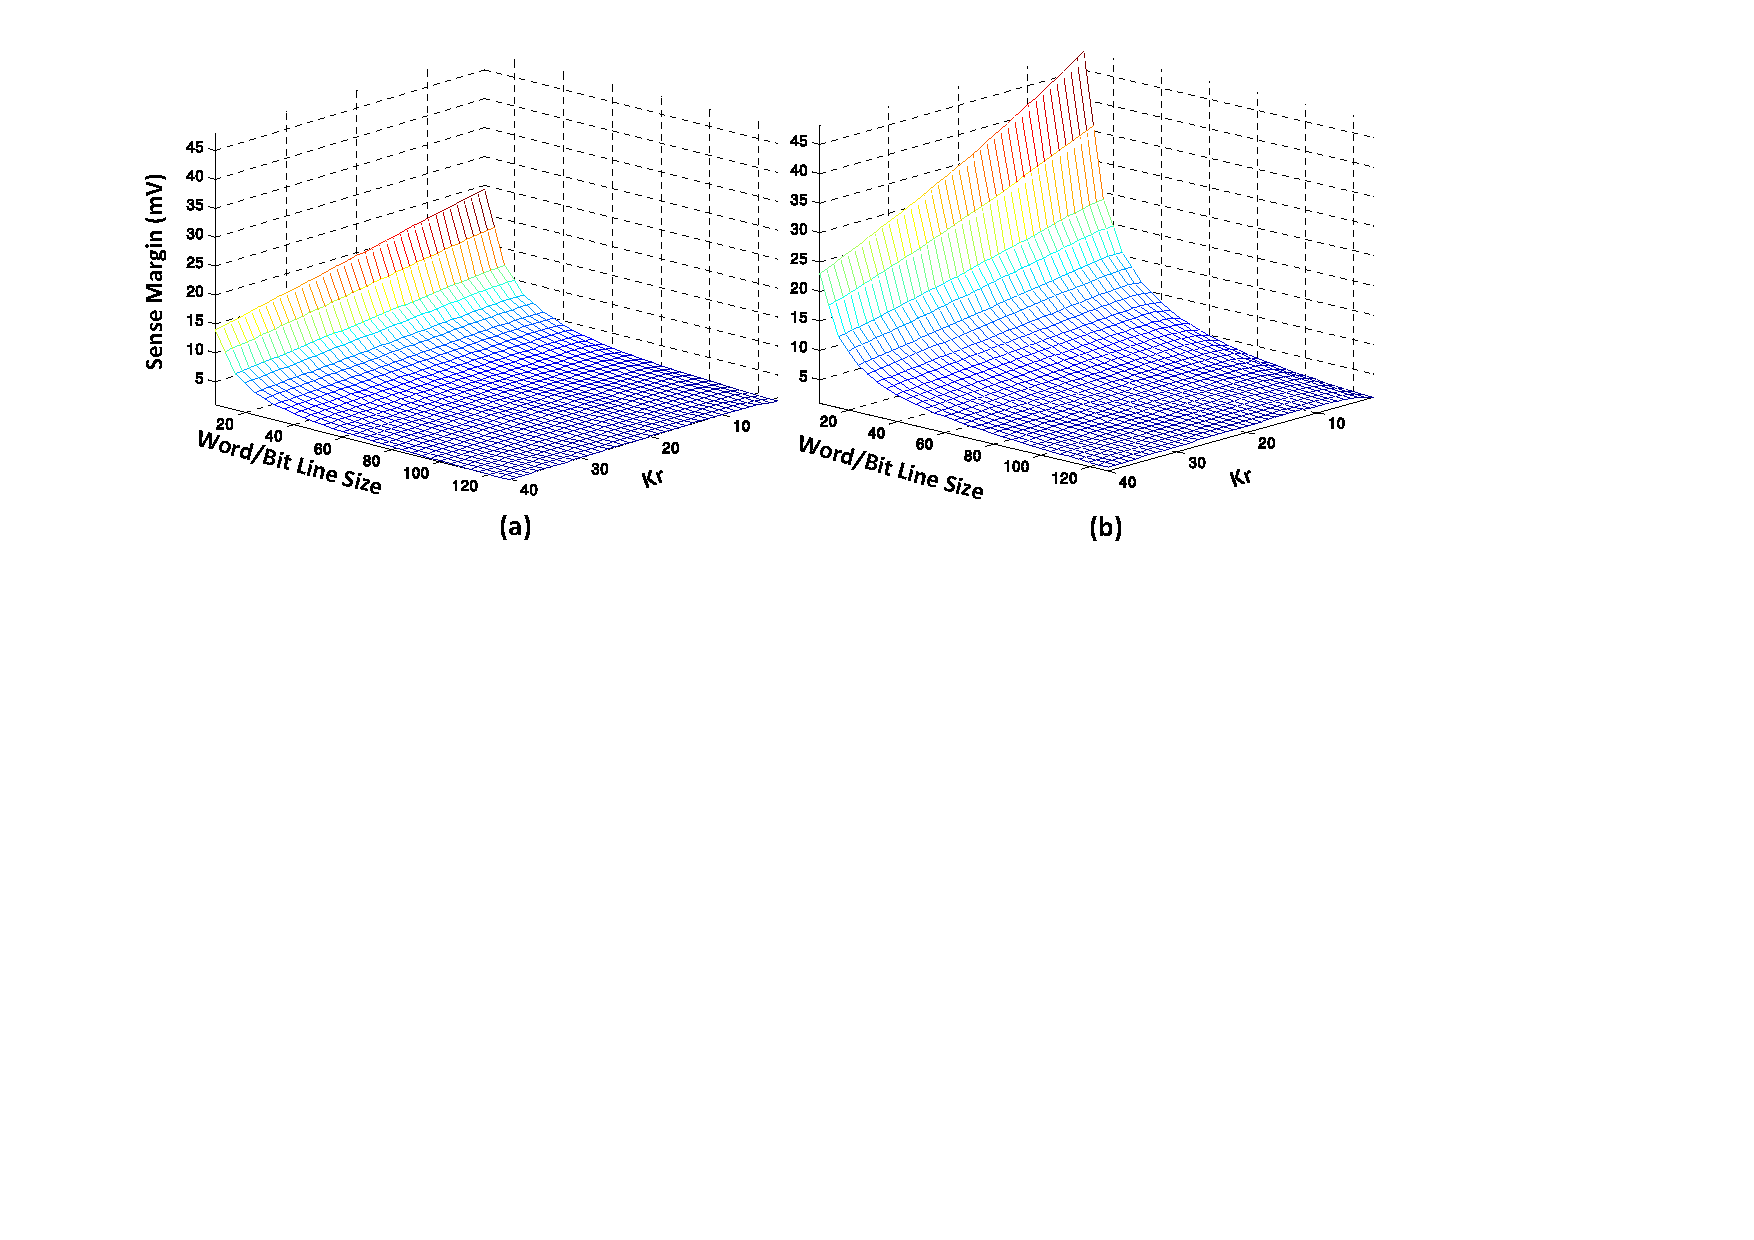
\includegraphics[width=0.5\textwidth]{./figures/sense_margin21}\\
%  \caption{The}\label{fig:sense_margin}
%\end{figure}

\begin{figure}[!t]
\centering
  % Requires \usepackage{graphicx}
  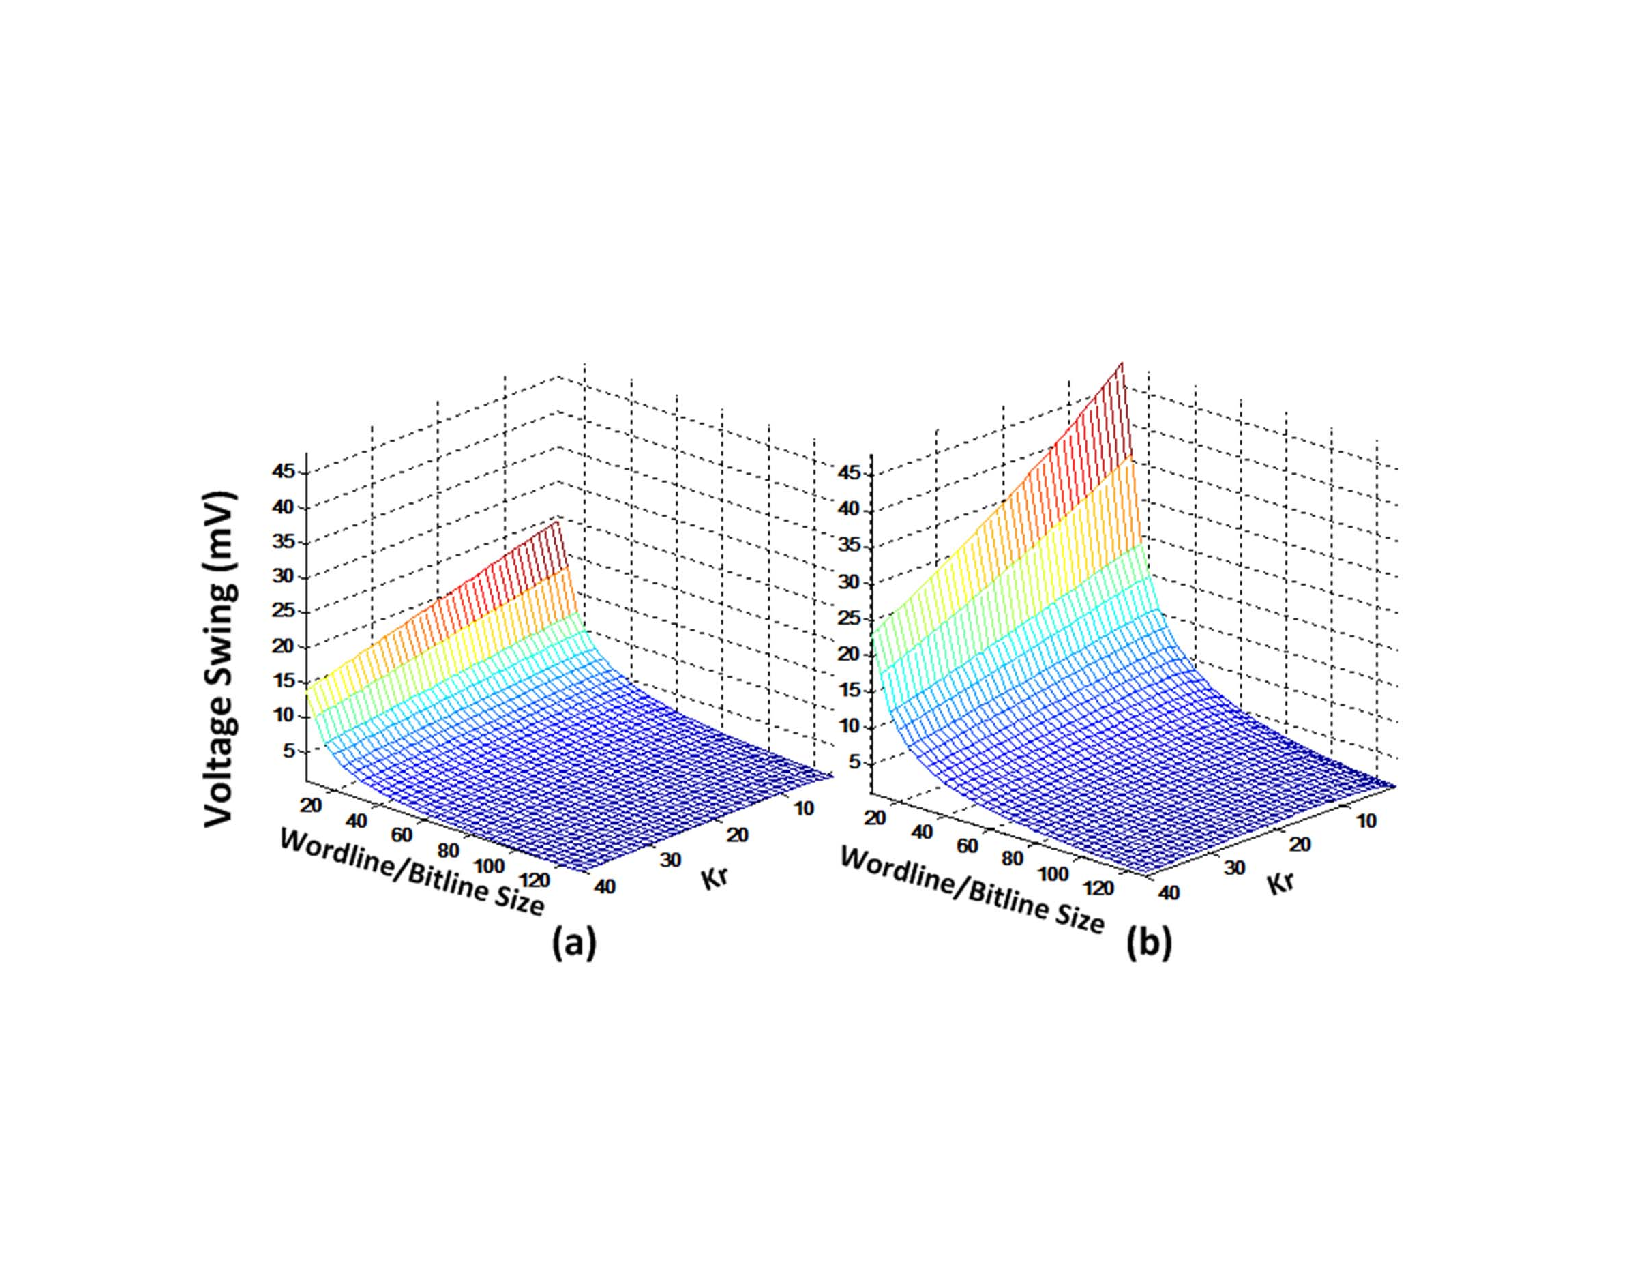
\includegraphics[width=0.5\textwidth]{./figures/sense_margin_f}\\
  \caption{Relationships among the voltage swing, array size and non-linearity. (a) Normal sensing scheme; (b) Two-step sensing scheme}\label{fig:sense_margin}
\end{figure}
